\begin{figure}[h]
    
    \centering
    \caption{How MRU performs against LRU given the trace: A, B, C, D, C}
    \label{fig:my_label}
    \scalebox{.85}{
\begin{tikzpicture} 
    \node[rounded corners,draw=black,label=above:MRU, minimum size=2cm] (a) at (0,0)  {
    \begin{tikzpicture}
        \node[rounded corners,draw=black,minimum size=0.8cm]{A};
    \end{tikzpicture}
    
\begin{tikzpicture}
        \node[rounded corners,draw=black,minimum size=0.8cm]{};
    \end{tikzpicture}
    
\begin{tikzpicture}
        \node[rounded corners,draw=black,minimum size=0.8cm]{};
    \end{tikzpicture}
    };
    \node[text width=3cm] at (-3, 0) 
    {Miss on A, A added to cache};

    
    \node[rounded corners,draw=black,minimum size=2cm] (b) at (0,-2.5)  {   
\begin{tikzpicture}
        \node[rounded corners,draw=black,minimum size=0.8cm]{A};
    \end{tikzpicture}
    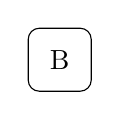
\begin{tikzpicture}
        \node[rounded corners,draw=black,minimum size=0.8cm]{B};
    \end{tikzpicture}
    
\begin{tikzpicture}
        \node[rounded corners,draw=black,minimum size=0.8cm]{};
    \end{tikzpicture}
    };
     \node[text width=3cm] at (-3,-2.5) 
    {Miss on B, B added to cache};
    
    \node[rounded corners,draw=black,minimum size=2cm] (c) at (0,-5)  {   
\begin{tikzpicture}
        \node[rounded corners,draw=black,minimum size=0.8cm]{A};
    \end{tikzpicture}
    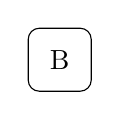
\begin{tikzpicture}
        \node[rounded corners,draw=black,minimum size=0.8cm]{B};
    \end{tikzpicture}
    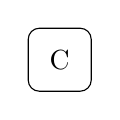
\begin{tikzpicture}
        \node[rounded corners,draw=black,minimum size=0.8cm]{C};
    \end{tikzpicture}
    };

    \node[text width=3cm] at (-3,-5) 
    {Miss on C, C added to cache};
      
    \node[rounded corners,draw=black,minimum size=2cm] (d) at (0,-7.5)  {   
\begin{tikzpicture}
        \node[rounded corners,draw=black,minimum size=0.8cm]{A};
    \end{tikzpicture}
    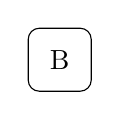
\begin{tikzpicture}
        \node[rounded corners,draw=black,minimum size=0.8cm]{B};
    \end{tikzpicture}
    
\begin{tikzpicture}
        \node[rounded corners,draw=black,minimum size=0.8cm]{D};
    \end{tikzpicture}
    };

     \node[text width=3cm] at (-3,-7.5) 
    {Miss on D, D added to cache, evict C since MRU};
    
    \node[rounded corners,draw=black,minimum size=2cm, below left=1 cm of d] (e) at (2.2,-8.4)  { 
    
\begin{tikzpicture}
        \node[rounded corners,draw=black,minimum size=0.8cm]{A};
    \end{tikzpicture}
    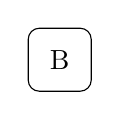
\begin{tikzpicture}
        \node[rounded corners,draw=black,minimum size=0.8cm]{B};
    \end{tikzpicture}
    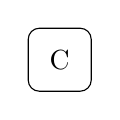
\begin{tikzpicture}
        \node[rounded corners,draw=black,minimum size=0.8cm]{C};
    \end{tikzpicture}
    };  

     \node[text width=2.5cm] at (-2.5,-9.8) 
    {Miss on C, evict D since MRU};
















    %LRU
    \node[rounded corners,draw=black,label=above:LRU, minimum size=2cm] (i) at (6,0)  {
    
\begin{tikzpicture}
        \node[rounded corners,draw=black,minimum size=0.8cm]{A};
    \end{tikzpicture}
    
\begin{tikzpicture}
        \node[rounded corners,draw=black,minimum size=0.8cm]{};
    \end{tikzpicture}
    
\begin{tikzpicture}
        \node[rounded corners,draw=black,minimum size=0.8cm]{};
    \end{tikzpicture}
    };
    \node[text width=3cm] at (10,0) 
    {Miss on A, A added to cache};
    \node[text width=3cm] at (4,0) 
    {\Huge A};

    
    \node[rounded corners,draw=black,minimum size=2cm] (j) at (6,-2.5)  {   
\begin{tikzpicture}
        \node[rounded corners,draw=black,minimum size=0.8cm]{A};
    \end{tikzpicture}
    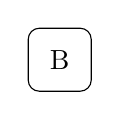
\begin{tikzpicture}
        \node[rounded corners,draw=black,minimum size=0.8cm]{B};
    \end{tikzpicture}
    
\begin{tikzpicture}
        \node[rounded corners,draw=black,minimum size=0.8cm]{};
    \end{tikzpicture}
    };
    \node[text width=3cm] at (10,-2.4) 
    {Miss on B, B added to cache};
    \node[text width=3cm] at (4,-2.4) 
    {\Huge B};
    
    \node[rounded corners,draw=black,minimum size=2cm] (k) at (6,-5)  {   
\begin{tikzpicture}
        \node[rounded corners,draw=black,minimum size=0.8cm]{A};
    \end{tikzpicture}
    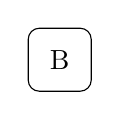
\begin{tikzpicture}
        \node[rounded corners,draw=black,minimum size=0.8cm]{B};
    \end{tikzpicture}
    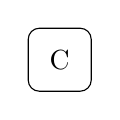
\begin{tikzpicture}
        \node[rounded corners,draw=black,minimum size=0.8cm]{C};
    \end{tikzpicture}
    };
    \node[text width=3cm] at (10,-4.8) 
    {Miss on C, C added to cache};
    \node[text width=3cm] at (4,-4.8) 
    {\Huge C};
    
      
    \node[rounded corners,draw=black,minimum size=2cm] (l) at (6,-7.5)  {   
\begin{tikzpicture}
        \node[rounded corners,draw=black,minimum size=0.8cm]{D};
    \end{tikzpicture}
    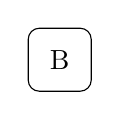
\begin{tikzpicture}
        \node[rounded corners,draw=black,minimum size=0.8cm]{B};
    \end{tikzpicture}
    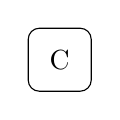
\begin{tikzpicture}
        \node[rounded corners,draw=black,minimum size=0.8cm]{C};
    \end{tikzpicture}
    };
     \node[text width=3cm] at (10,-7.4) 
    {Miss on D, D added to cache, Evict A since LRU};
    \node[text width=3cm] at (4,-7.4) 
    {\Huge D};

    
    \node[rounded corners,draw=black,minimum size=2cm, below left=1 cm of l] (m) at (8.2,-8.4)  { 
    
\begin{tikzpicture}
        \node[rounded corners,draw=black,minimum size=0.8cm]{D};
    \end{tikzpicture}
    
\begin{tikzpicture}
        \node[rounded corners,draw=black,minimum size=0.8cm]{A};
    \end{tikzpicture}
    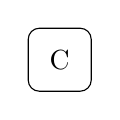
\begin{tikzpicture}
        \node[rounded corners,draw=black,minimum size=0.8cm]{C};
    \end{tikzpicture}
    };  
    \node[text width=3cm] at (10,-10) 
    {Hit on C};
    \node[text width=3cm] at (4,-10) 
    {\Huge C};


    \draw[thick,->] (a) -- (b);
    \draw[thick,->](b) -- (c);  
    \draw[thick,->](c) -- (d);  
    \draw[thick,->](d) -- (e);  

    
    \draw[thick,->] (i) -- (j);
    \draw[thick,->](j) -- (k);  
    \draw[thick,->](k) -- (l);  
    \draw[thick,->](l) -- (m);  
\end{tikzpicture}
}
\end{figure}